\chapter{Methodology}

In this chapter it is going to be explained all the steps required to achieve a functional neural network to participate at the ActivityNet Challenge. For this challenge there was no baseline because video tasks have not been faced on the group I did this project, so was required to face the challenge from zero.

\section{ActivityNet Dataset}

The ActivityNet Dataset\cite{caba2015activitynet} is \textit{A Large-Scale Video Benchmark for
Human Activity Understanding}. This dataset, on version 1.3 which is the one used for the challenge, contains 19,994 videos with a different 200 activities labeled which represents a wide range of human activities. In total there are 660 hours of video and the subsets are split on the following way: 50\% training dataset, 25\% validation dataset and 25\% testing dataset. Each video of the dataset have an activity happening in there and one or more annotations saying in which temporal locations the activity is happening.

All the video from this dataset are placed on \textit{YouTube} so only the links for the video are provided because of copyright issues. So the first task to be done was download all the videos on our own. This was done using a program called \textit{youtube-dl} which allows to download videos from that platform. But some videos show up with some issues as all of them were stored on a third party platform. This issues went from some of them presenting location restrictions to some of them  even were removed by their owners. This let only download 19,811 video which considering the size of the dataset, was not a big deal.

Once all the videos from the dataset were downloaded, the number of frames of each video was extracted because the temporal unit at the time to process it will be the frames. In addition to this, some stats were computed. Such as the whole number of frames from all the videos in the dataset which is 65.6 million frames. Also, the lenght in minutes of each activity at the dataset was plot on Figure~\ref{fig:dataset_stats} to have an idea about the activities frequencies. As can be seen, not all the activities have the same appearance along the dataset, varying from 40 minutes the least frequent activity to 3.5 hours the more frequent one. In total over all the dataset there are 313 hours of activities which will be required to detect and localize.

\begin{figure}
\begin{center}
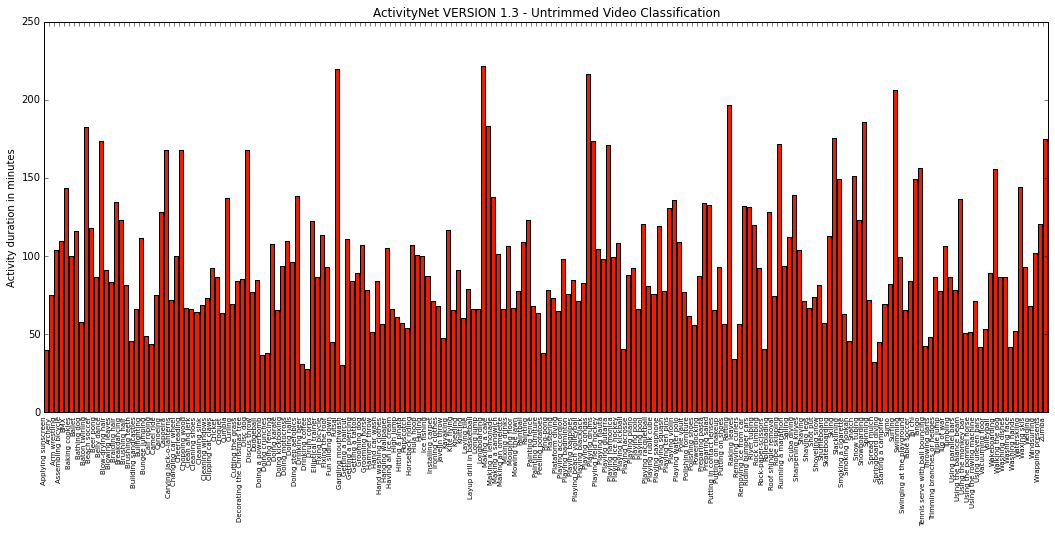
\includegraphics[width=1\linewidth]{img/methodology/dataset_stats}
\end{center}
\caption{Activity duration in minutes for each activity on the dataset}
\label{fig:dataset_stats}
\end{figure}

\section{Extracting Video Features Using C3D}

The C3D network\cite{tran2014learning} was decided to use as a video features extractor to be known to extract very well either spatial and temporal correlations from videos.
%%TODO add references
The original paper proposing and studying 3D convolutions applied to videos, also give code to reproduce it. The code given was based on a version of \textit{Caffe}\cite{jia2014caffe} dated to 2014. Because the code to use 3D convolutions did not support last functionalities and did not work with the \textit{Python} environment used for this project, the model trained with C3D and the Sports1M dataset was ported to \textit{Keras}\footnote{All the process has been open sourced and can be found in: \url{https://gist.github.com/albertomontesg/d8b21a179c1e6cca0480ebdf292c34d2}}. Keras is a deep learning framework that works over \textit{Theano}\cite{theano2016theano} and \textit{TensorFlow}\cite{abadi2016tensorflow}, two computational frameworks which allow run and train deep learning models over either CPU and GPU.



Then how the videos were read (OpenCV) and passed to the ported C3D model. Extracted the features of the fc6 layer.

\section{Extracting Audio Features}

The audio features extracted: MFCC and Spectral

\section{Prepare the Data for Stateful Recurrent Networks}

How the data was prepared to be trained to the Recurrent Network

\section{Networks Configuration}

Talk about the different configurations I have tried:
\begin{itemize}
    \item Normal LSTM with different variations in number of layers and neurons
    \item Feedback Model
    \item Semisupervised
\end{itemize}

\section{Post-Processing Proposed}

How to compute the classification for each video.

How to get the temporal localization of the activities to the videos.
Mean filter, activity probability computation.
